\documentclass[11pt]{article}
\usepackage[letterpaper]{geometry}

%Used to split pages into two columns, IE the truth tables
\usepackage{multicol}

%Used to place figures
\usepackage{graphicx}
\usepackage{float}

%Used so that multi-line caption text is centered instead of left-aligned
\usepackage[center]{caption}

%Used to squish TOC
\usepackage{setspace}

%Used to show code nicely formatted
\usepackage{listings}
\usepackage{color}
\usepackage{placeins}

%Used for Showing Mathematical Proofs
\usepackage{amsmath,amsthm,amssymb}

%Used for tables
\usepackage{array}
\usepackage{booktabs}

%Used for canceling terms in Math
\usepackage{cancel}

\usepackage{enumitem}

%Used to strike out items
\usepackage[normalem]{ulem}

\definecolor{dkgreen}{rgb}{0,0.6,0}
\definecolor{gray}{rgb}{0.5,0.5,0.5}
\definecolor{mauve}{rgb}{0.58,0,0.82}

\lstset{frame=tb,
	language=Java,
	aboveskip=3mm,
	belowskip=3mm,
	showstringspaces=false,
	columns=flexible,
	basicstyle={\small\ttfamily},
	numbers=none,
	numberstyle=\tiny\color{gray},
	keywordstyle=\color{blue},
	commentstyle=\color{dkgreen},
	stringstyle=\color{mauve},
	breaklines=true,
	breakatwhitespace=true,
	tabsize=3
}

%Used to include the signatures sheet
\usepackage{pdfpages}

\title{EENG-331 Lab 5:\linebreak \linebreak CS stage Design and Audio Processing}
\author{Jeremy Munson}
\geometry{top=.8in, bottom=.8in, left=.8in, right=.8in}

\setlength{\parindent}{0em}
\setlength{\parskip}{.5em}
\setlength{\floatsep}{20px}
\setlength{\textfloatsep}{20px}

\begin{document}
    \null \hfill May 18, 2024\linebreak
    \null \hfill Jeremy Munson\linebreak
    \null \hfill Corbin Cole\linebreak
    
    \makebox[\textwidth]{\textbf{\huge EENG-331 Lab 5:}}

    \makebox[\textwidth]{\textbf{\large SPICE Netlist Simulation}}
    \vspace{-20px}
	\section{Prelab}
		\FloatBarrier
		\vspace{-5px}
	
	\subsection{Common Source Amplifier With Resistor Biasing and Passive Load}
		Prior to the lab, each team member designed a Common Source Stage with resistor divider biasing and resistor load, for $A_v = 10$, $5mW$ power budget, $V_{ov} = 100mV$, $k_p = \frac{100\mu A}{V^2}$, $V_{dd} = 5V$, $\lambda = 0$, and $V_{th} = 0.5V$. Additionally, it was assumed that an "investment" of 10\% of the power budget on setting the gate voltage was intended. Finally, we assumed that $L = 10\mu m$ is the smallest allowable value for the design. The hand-calculations for this amplifier design can be seen in Figure(\ref{fig:prelab1}). The resulting design has values as follows:\\
		\begin{align}
			\label{eqn:CS_POW_ID} &P_{\text{ower consumed by } I_d} = 90\% \cdot 5mW &=& 4.5mW \\
			\label{eqn:CS_ID} &I_d = \frac{4.5mW}{5v} &=& 0.9mA \\
			\label{eqn:CS_WL} I_d = 0.9mA = \frac{1}{2} k_p \frac{W}{L} V_{ov}^2 \rightarrow &\frac{W}{L} &= \frac{18000\mu}{10\mu} =& 1800 \\
			\label{eqn:CS_gm} &g_m = \frac{2I_d}{V_{ov}} &=& 18mS \\
			\label{eqn:CS_RD} A_v = -g_mR_d \rightarrow |A_v| = g_mR_d \rightarrow &R_d &=& 556 \Omega \\
			\label{eqn:CS_VG} &V_{g,dc} = V_{th} + V_{ov} &=& 0.6v \\
			\label{eqn:CS_GATE_BIAS} &I_{\text{gate voltage divider}} = \frac{10\% \cdot 5mW}{5v} &=& 0.1mA \\
			\label{eqn:CS_R2} &R_2 = \frac{0.6V}{0.1mA} &=& 6k\Omega \\
			\label{eqn:CS_R1} &R_1 = \frac{5V - 0.6V}{0.1mA} &=& 44k\Omega
		\end{align}

	\subsection{Common Source Amplifier With Self-Biasing, Active Load}
		Additionally, a CS stage was designed using a current source for the load, and the self-biasing method for setting the gate voltage. This stage follows all the same constraints as the previous section.
		
		Regarding $I_d$, the instructions say to use the same $I_d$ as the previous stage. This would be only $0.9mA$, and also did not seem to be in alignment with email communications received about the lab calculations. We instead chose to interpret this as "Use the same power budget", which results in $I_d = 1mA$, and is consistent with the other communications received.
		
		Before presenting the calculations, know that an oversight was made on the gain of the stage initially, but quickly corrected after the start time of the lab. Since the prelab was due at the start of the lab, we present the initial flawed calculations in the scan of the prelab, but the correct calculations in this lab report. The flawed calculations can be seen in Figure(\ref{fig:prelab2}).
		
		The mistake made was to take the gain equation for CS w/ active load, $A_v = g_m r_o$, and use it with $\lambda = 0$, but mistakenly behave as if \cancel{$r_o = 1$} in that case, which gave \cancel{$A_v = g_m$}, suggesting a need for a very large $g_m$. It is believed that a contributing factor to the mistake was the nonsensical correct result: $r_o = \infty$, which is fine, but $A_v = g_m \cdot \infty = \infty$, which would make it impossible to meet the $A_v = 10$ constraint.
		
		The calculations for this stage are much more simple. Self-biasing will set $V_g$. We simply need to choose $\frac{W}{L}$ such that $V_{ov} = 0.1$, to match the constraint. We take Equation(\ref{eqn:CS_WL}), and recalculate $\frac{W}{L}$ for $I_d = 1mA$, returning Equation(\ref{eqn:SB_WL}).
		\begin{align}\label{eqn:SB_WL} I_d = 1mA = \frac{1}{2} k_p \frac{W}{L} V_{ov}^2 \rightarrow \frac{W}{L} = \frac{20000\mu}{10\mu} = 2000 \end{align}
		
		
		The choice of $R_g$ is arbitrary, but it is worth noting that $R_g$ results in coupling between $V_{in}$ and $V_{out}$. Since a CS stage is an inverting amplifier, this makes the coupling a negative feedback to the input, degrading our overall gain. In our simulations we are using a voltage source with no series resistance for $V_{in}$; as a result this effect is not seen except as an interaction with the input coupling capacitor, which we can suppress by making the capacitor arbitrarily large.
		
	\begin{figure}
		\centering
		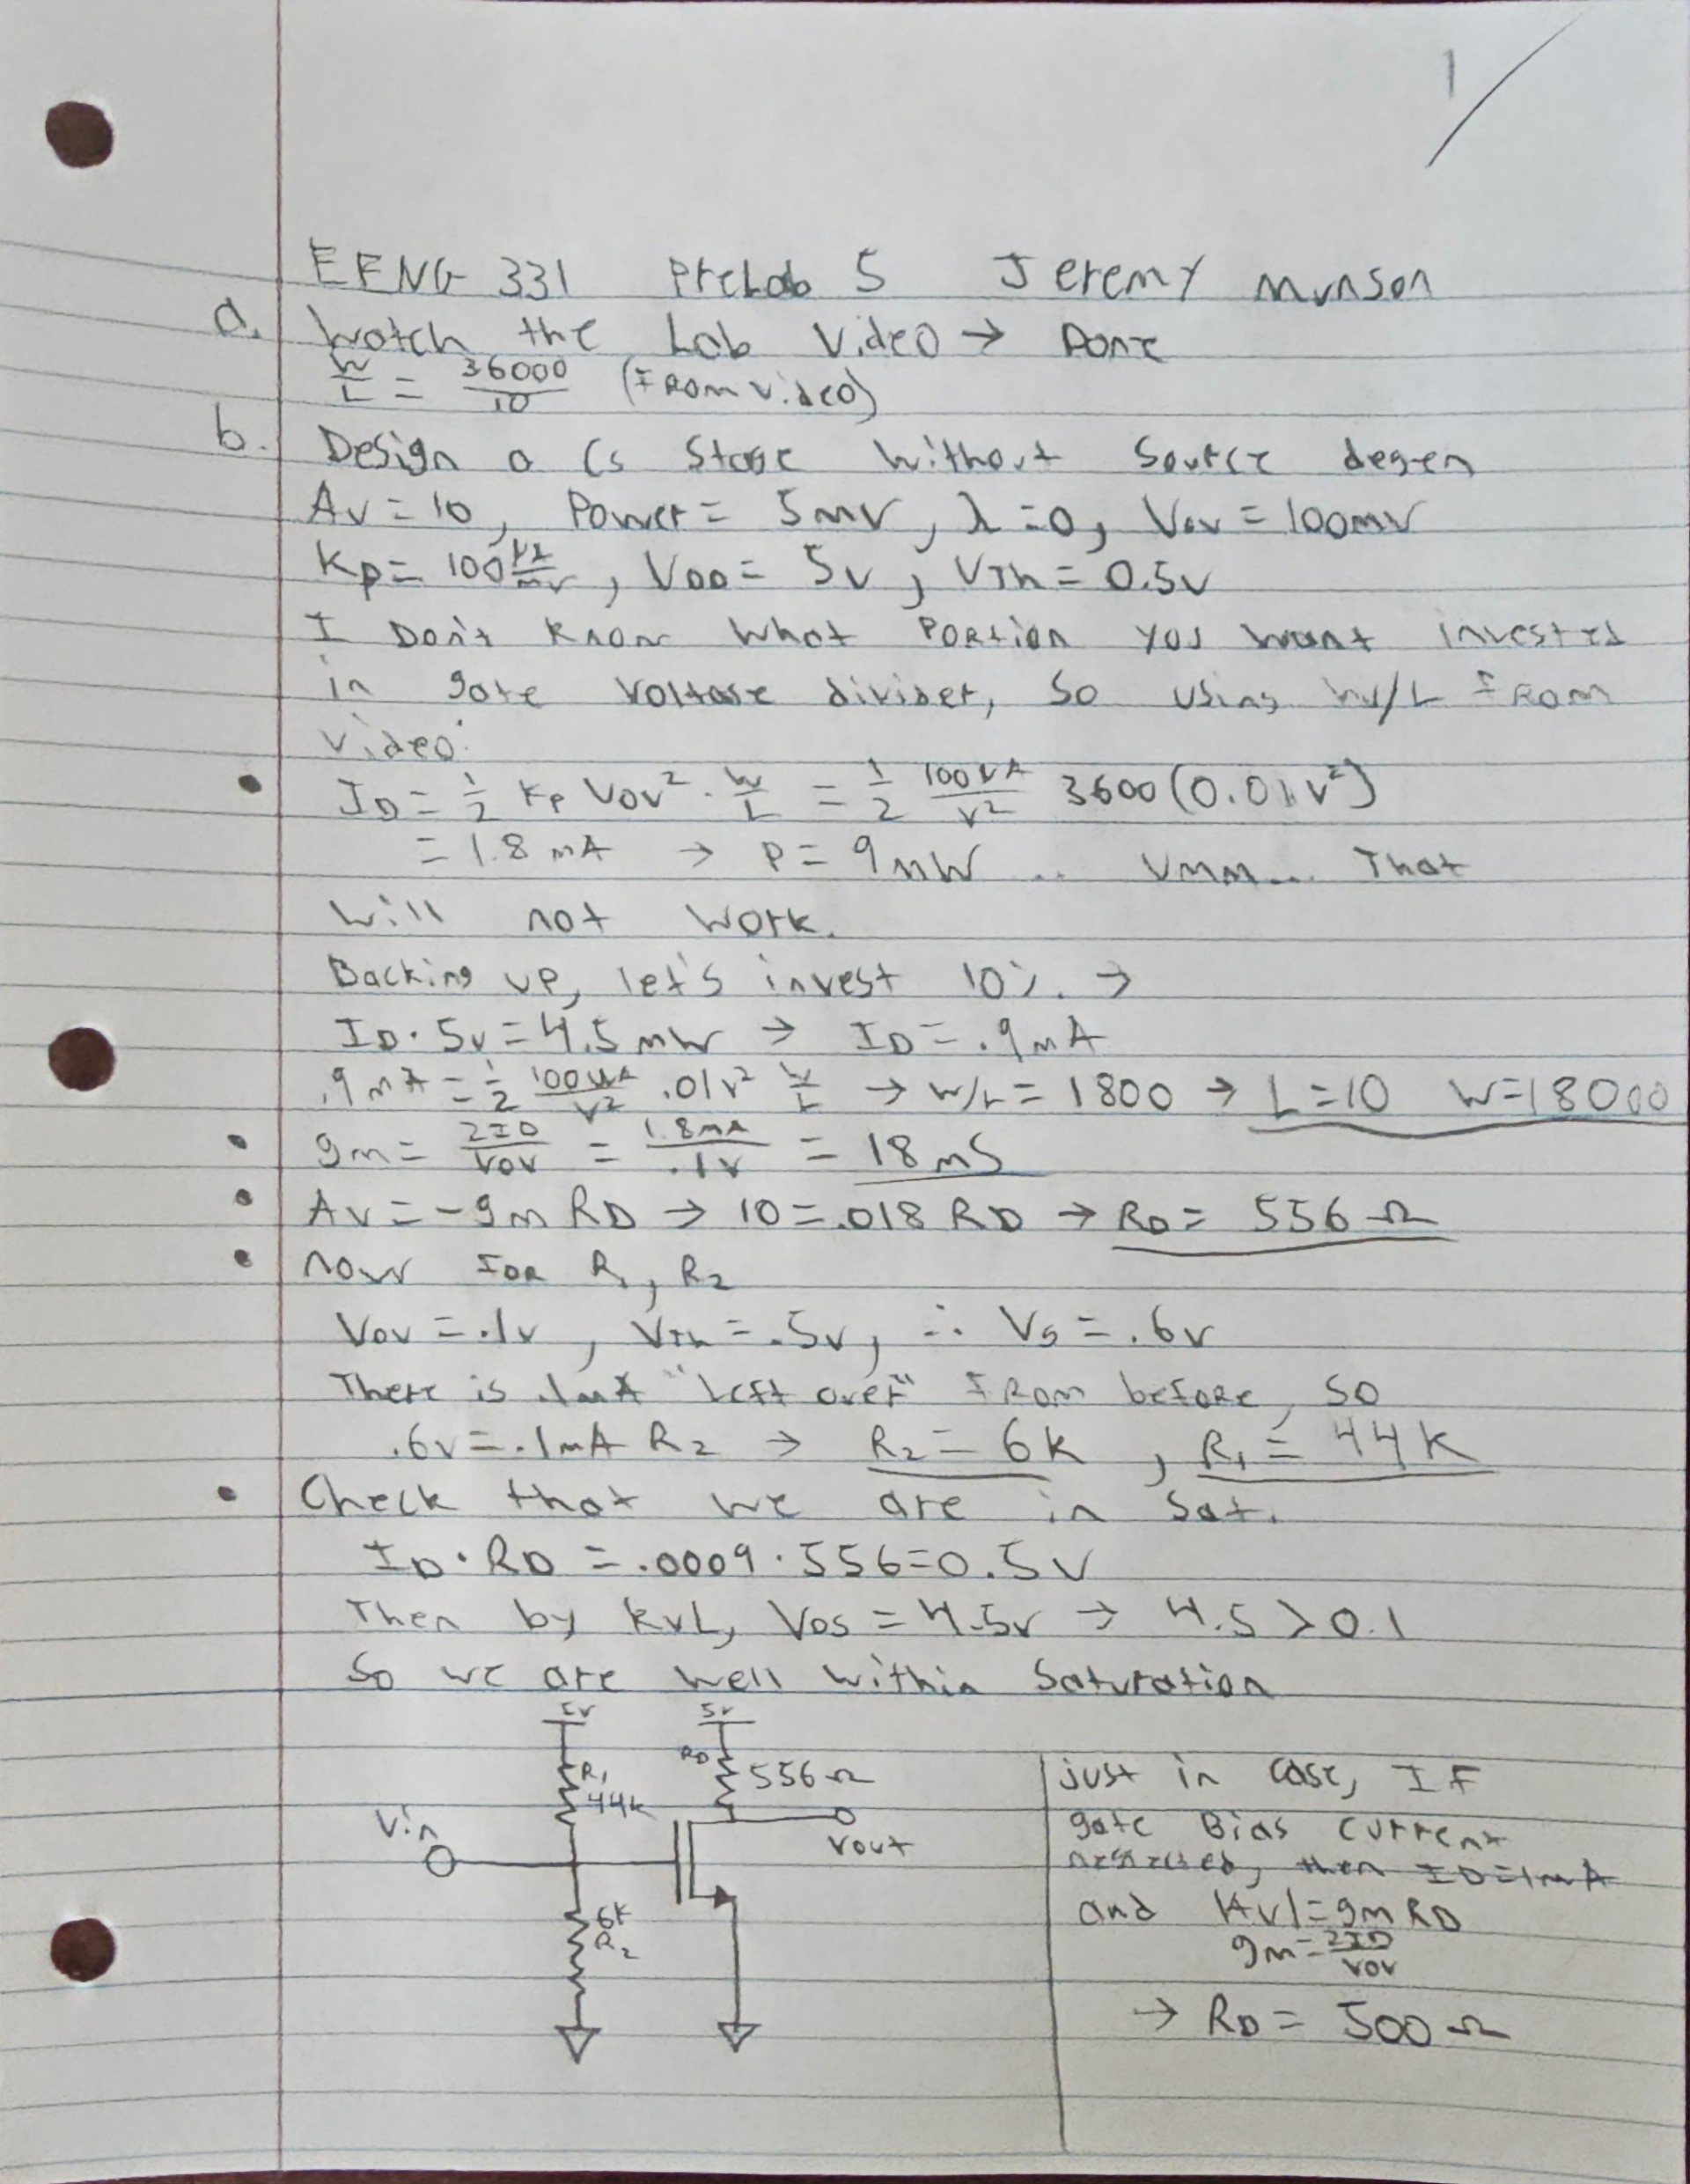
\includegraphics[width=0.95\linewidth]{prelab1}
		\caption{Prelab Calculations for CS amplifier with resistor load \& biasing}
		\label{fig:prelab1}
	\end{figure}

	\begin{figure}
	\centering
		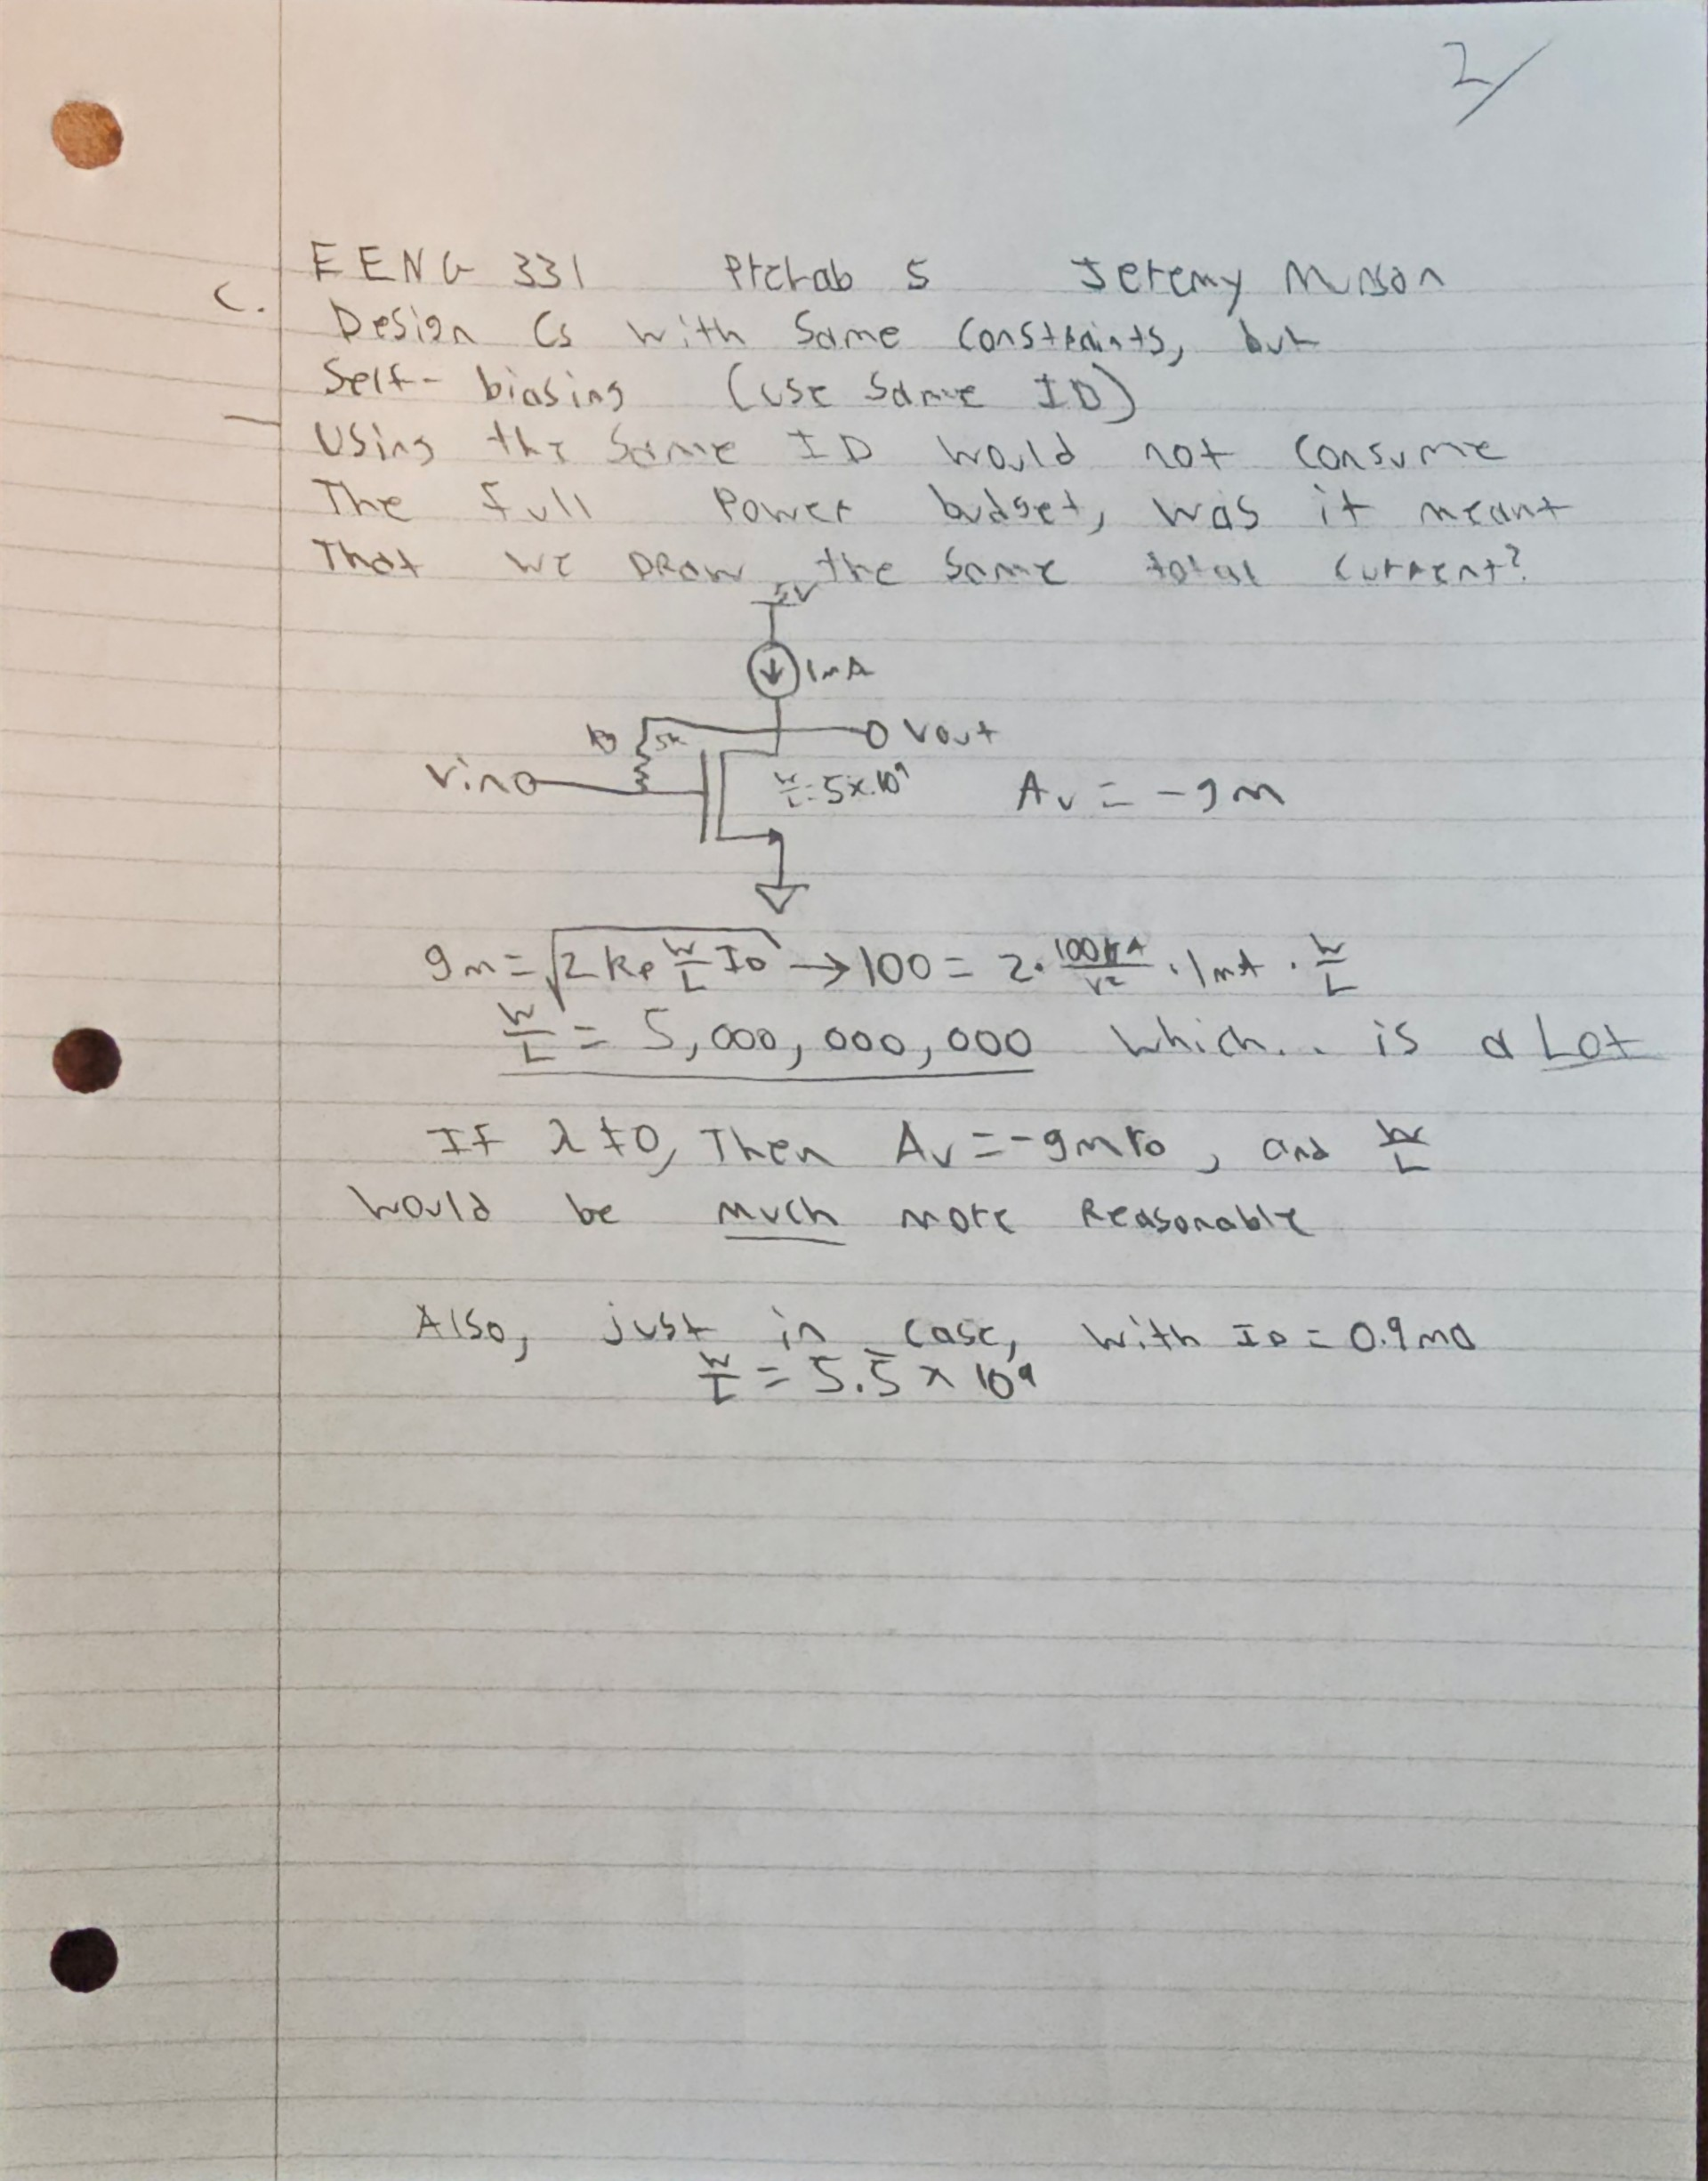
\includegraphics[width=0.95\linewidth]{prelab2}
		\caption{Mistaken Prelab Calculations for CS amplifier w/ active load and self-biasing}
		\label{fig:prelab2}
	\end{figure}

\FloatBarrier
	
	\newpage
	\addcontentsline{toc}{section}{Table Of Contents}
	\setcounter{tocdepth}{2}
	\begin{spacing}{0.1}
		\tableofcontents
		\listoffigures
	\end{spacing}

\end{document}